
\section{\unit{GridParticles}}
\label{Sec:GridParticles}

Flash-X is primarily an Eulerian code, however, there is support for
tracing the flow using Lagrangian particles. In \flashx we have
generalized the interfaces in the Lagrangian framework of the Grid
unit in such a way that it can also be used for miscellaneous 
non-Eulerian data such as tracing the path of a ray through the domain, 
or tracking the motion of solid bodies immersed in the fluid. Flash-X also
uses active particles with mass in cosmological simulations, and
charged particles in a hybrid PIC solver. Each particle has an
associated data structure, which contains fields such as its physical
position and velocity, and relevant physical attributes such as mass
or field values in active  particles. Depending upon the time advance
method, there may be other fields to store intermediate values. Also,
depending upon the requirements of the simulation, other physical variables
such as temperature \etc~ may be added to the data structure.
The \unit{GridParticles} subunit of the \unit{Grid} unit has two
sub-subunits of its own. The \unit{GridParticlesMove} sub-subunit 
moves the data structures associated with individual particles when
the particles move between blocks; the actual movement of the
particles through time advancement is the responsibility of the
\unit{Particles} unit. Particles move from one block to another
when their time advance places them outside their current
block. In AMR, the particles can also change their block through the
process of refinement and derefinement. The \unit{GridParticlesMap}
sub-subunit provides mapping between particles data and the mesh
variables. The mesh variables are either cell-centered or
face-centered, whereas a particle's position could be anywhere in the
cell. The \unit{GridParticlesMap} sub-subunit calculates the particle's
properties at its position from the corresponding mesh variable values
in the appropriate cell . When using active particles, this sub-subunit
also maps the mass of the particles onto the specified mesh variable
in appropriate cells.   The next sections describe the
algorithms for moving and mapping particles data.


\subsection{GridParticlesMove}
\label{Sec:GridParticlesMove}
\flashx has implementations of three different parallel algorithms
for moving the particles data when they are displaced from their
current block. \flashx had an additional algorithm, \code{Perfect
  Tree Level} which made use of the oct-tree structure. However,
because in all performance experiments it performed significantly
worse than the other two algorithms, it is not supported currently in
\flashx. The simplest algorithm, \code{Directional algorithm} is  
applicable only to the uniform grid when it is configured with one
block per processor. This algorithm uses directional movement of data,
and is easy because the directional neighbors are trivially known. 
The movement of particles data is much more challenging with AMR even
when the grid is not refining. Since the blocks are at various
levels of refinement at any given moment, a block may have more than one
neighbor along one or more of its faces. The distribution of blocks
based on space-filling curve is an added complication since the
neighboring blocks along a face may reside at a non-neighboring processor
The remaining two algorithmss included in \flashx implement
\code{GridParticlesMove} subunit for the adaptive mesh;  \code{Point
 to Point} and \code{Sieve}, of which only the \code{Sieve} algorithm
is able to move the data when the mesh refines. Thus even when a user
opts for the \code{PointToPoint} implementation for moving particles
with time evolution, some part of the \code{Sieve} implementation must
necessarily be included to  successfully move the data upon
refinement.   

\subsubsection{Directional Move}
\label{Sec: ug_algorithm}
The Directional Move algorithm for moving particles in a Uniform Grid 
minimizes the number of communication steps instead of minimizing
the volume of data moved. Its implementation has the following steps:
\begin{enumerate}
\item Scan particle positions.  Place all particles with their $x$
coordinate value greater than the block bounding box in the Rightmove
bin, and place those with $x$ coordinate less than block bounding box in
Leftmove bin.
\item Exchange contents of Rightbin with the right block neighbor's Leftbin
contents, and those of the Leftbin with left neightbor's Rightbin
contents.
\item Merge newly arrived particles from step 2 with those which did not move outside their original block.
\item Repeat steps 1-3 for the y direction.
\item Repeat step 1-2 for the z direaction.
\end {enumerate}

At the end of these steps, all particles will have reached their
destination blocks, including those that move to a neighbor on the
corner. \figref{Fig:ugMoveParticle} illustrates the steps in getting
a particle to its correct destination.
\begin{figure}
\begin{center}
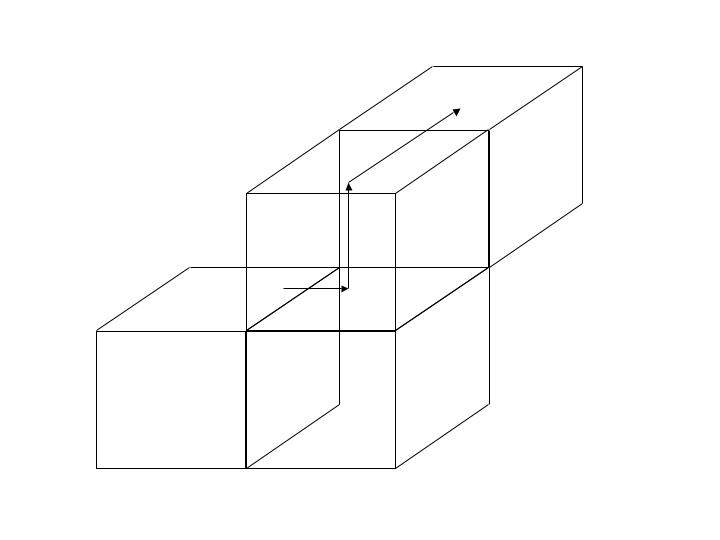
\includegraphics[width=3in]{Grid_ugMoveParticle}
\caption{\label{Fig:ugMoveParticle}
        Moving one particle to a neighbor on the corner.}
\end{center}
\end{figure}

\subsubsection {Point To Point Algorithm}
\label {Sec: ptop_algorithm}
A bitmap of the mesh maintained by the Bittree algorithm has complete
information about the neighborhood of all the blocks on a
processor. Thus it is possible to determine the
processor and block number of the destination block for each particle.
The PointToPoint implementation finds out the destinations for every
particles that is getting displaced from its block. Particles going to
local destination blocks are moved first. The remaining particles are
sorted based on their destination processor number, followed by a
couple of global operations that allow every processor to determine
the number of particles it is expected to receive from all of the
other processors. A processor then posts asynchronous receives for
every source processor that had at least one particle to send to
it. In the next step, the processor cycles through the sorted list of
particles and sends them to the appropriate destinations using
synchronous mode of communition. 

